
\documentclass{article}
\usepackage{amsmath}
\usepackage[utf8]{inputenc}
\usepackage{ctex}
\usepackage{indentfirst}

\usepackage{graphicx}

\usepackage{listings}
\usepackage{color}

\lstset{
    language=Python, % 设置语言
    basicstyle=\ttfamily, % 基本字体样式
    keywordstyle=\color{blue}, % 关键词的颜色
    commentstyle=\color{green}, % 注释的颜色
    stringstyle=\color{red}, % 字符串的颜色
    showstringspaces=false, % 不显示字符串间隙
    numbers=left, % 显示行号
    numberstyle=\tiny\color{gray}, % 行号样式
    breaklines=true, % 自动换行
    frame=single % 给代码框加一个边框
}


\setlength{\parindent}{2em}

\begin{document}

\begin{center}
    \Large \textbf{Lab3 实验报告}\\
    \vspace{1em}
    姓名:~~学号:~~班级:
\end{center}

\section{实验概览}

    本次实验主要学习了SIFT算法和其在图像匹配上的应用

    SIFT算法是David Lowe于1999年提出的局部特征描述子,并于2004年进行了更深入的发展和完善。
    Sift特征匹配算法可以处理两幅图像之间发生平移、旋转、仿射变换情况下的匹配问题,具有很强的匹配能力。总体来说,SIFT算子具有以下特性:

    1.SIFT特征是图像的局部特征,对平移、旋转、尺度缩放、亮度变化、遮挡和噪声等具有良好的不变性,对视觉变化、仿射变换也保持一定程度的稳定性。

    2.独特性好,信息量丰富,适用于在海量特征数据库中进行快速、准确的匹配。

    3.多量性,即使少数的几个物体也可以产生大量SIFT特征向量。

    4.速度相对较快,经优化的Sift匹配算法甚至可以达到实时的要求。

    5.可扩展性强,可以很方便的与其他形式的特征向量进行联合。

    SIFT算法的实质是在不同的尺度空间上查找关键点(特征点),并计算出关键点的方向。
    SIFT所查找到的关键点是一些十分突出,不会因光照,仿射变换和噪音等因素而变化的点,如角点、边缘点、暗区的亮点及亮区的暗点等。

    SIFT算法主要步骤:

a.检测尺度空间关键点

b.精确定位关键点

c.为每个关键点指定方向参数

d.关键点描述子的生成

\section{练习题的解决思路}

\subsection{图像关键点提取——高斯金字塔方法}

\subsubsection{高斯金字塔}




    尺度空间使用高斯金字塔表示。Tony Lindeberg指出尺度规范化的LoG
    (Laplacion of Gaussian)算子具有真正的尺度不变性,
    Lowe使用高斯差分金字塔近似LoG算子,在尺度空间检测稳定的关键点。
    尺度空间的表示如下:

对原图像 \( I(x, y) \) 建立尺度空间 \( L(x, y, \sigma) \) 的方法是将图像 \( I(x, y) \) 与高斯核 \( G(x, y, \sigma) \) 卷积:
\[
L(x, y, \sigma) = G(x, y, \sigma) * I(x, y)
\]

其中 \( G(x, y, \sigma) \) 是高斯卷积核:
\[
G(x, y, \sigma) = \frac{1}{2\pi\sigma^2} e^{-\frac{x^2 + y^2}{2\sigma^2}}
\]

将两个不同尺度的 \( L \) 相减可得到高斯差分图像:
\[
D(x, y, \sigma) = (G(x, y, k\sigma) - G(x, y, \sigma)) * I(x, y)
= L(x, y, k\sigma) - L(x, y, \sigma)
\]

构建 \( D(x, y, \sigma) \) 是为了检测尺度空间极值点。

    为了让尺度体现其连续性,在简单下采样的基础上加上了高斯滤波。一幅图像可以产生几组图像,一组图像包括几层图像。
    高斯金子塔的构建过程可分为两步:

    1.对图像做高斯平滑;

    2.对图像做降采样

    根据论文内容,实际实现与手册/ppt描述略有不同。对于给定的照片,假定其已进行了\(\sigma = 0.5\)的高斯模糊,
    首先将其拉伸至原本的两倍,这一步通过插值填补缺失的像素值。此时其对应的\(\sigma' =  0.5 \times 2 = 1\).
    原文取\(\sigma_0 = 1.6\), 由高斯模糊的性质(即对一个图像先后做\(\sigma_1, \sigma_2\)的高斯模糊等于做
    \(\sigma = \sqrt{\sigma_1^2 + \sigma_2^2}\)的高斯模糊),需要再进行一次\(\sigma'' = \sqrt{1.6 * 1.6 - 1 * 1}\)
    的高斯模糊,得到第一组第一张图像。

    随后取\(k = 2^{\frac{1}{3}}\), 根据上述高斯模糊的性质生成每组的第2至6层图像。由论文内容,取第四张(也就是每组倒数第三张)
    降采样后作为下一组的第一张图像。降采样的操作为提取原图像所有偶数坐标的点,连接后得到原图像分辨率\(\frac{1}{4}\)的新图像。

    与手册/ppt描述不同的是,由于降采样会导致新图像的高斯模糊等效为原本的一半,这里每组同一层图像的高斯模糊值都应该相等,而非描述中
    组间差距2倍。同样取层间高斯模糊的比例为\(k\),重复上述操作,最后得到6组6层图像。

    这里,组数6由\(\log_2(min{H, W} - 3)\)得到,其中\(H, W\)代表初始图像的高和宽。
    层数选取将在下一节中解释。

\begin{figure}[h]
\centering
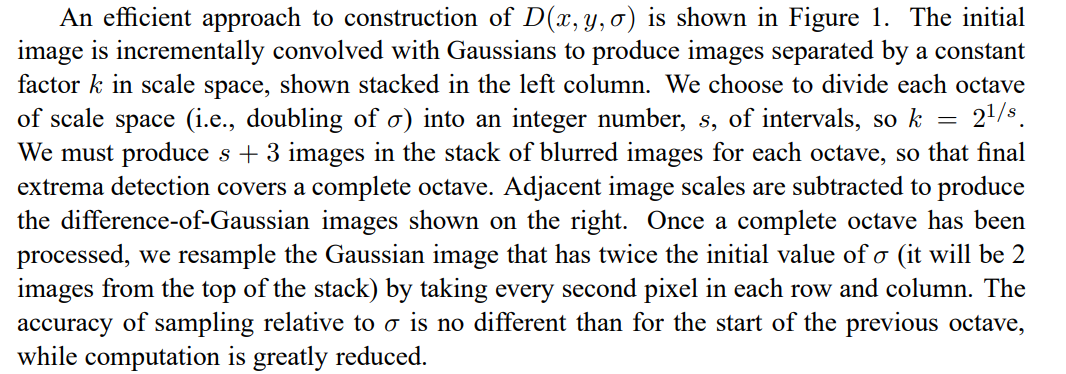
\includegraphics[width=1\textwidth]{./others/a1}
\caption{论文原文1}
\end{figure}

\begin{figure}[h]
\centering
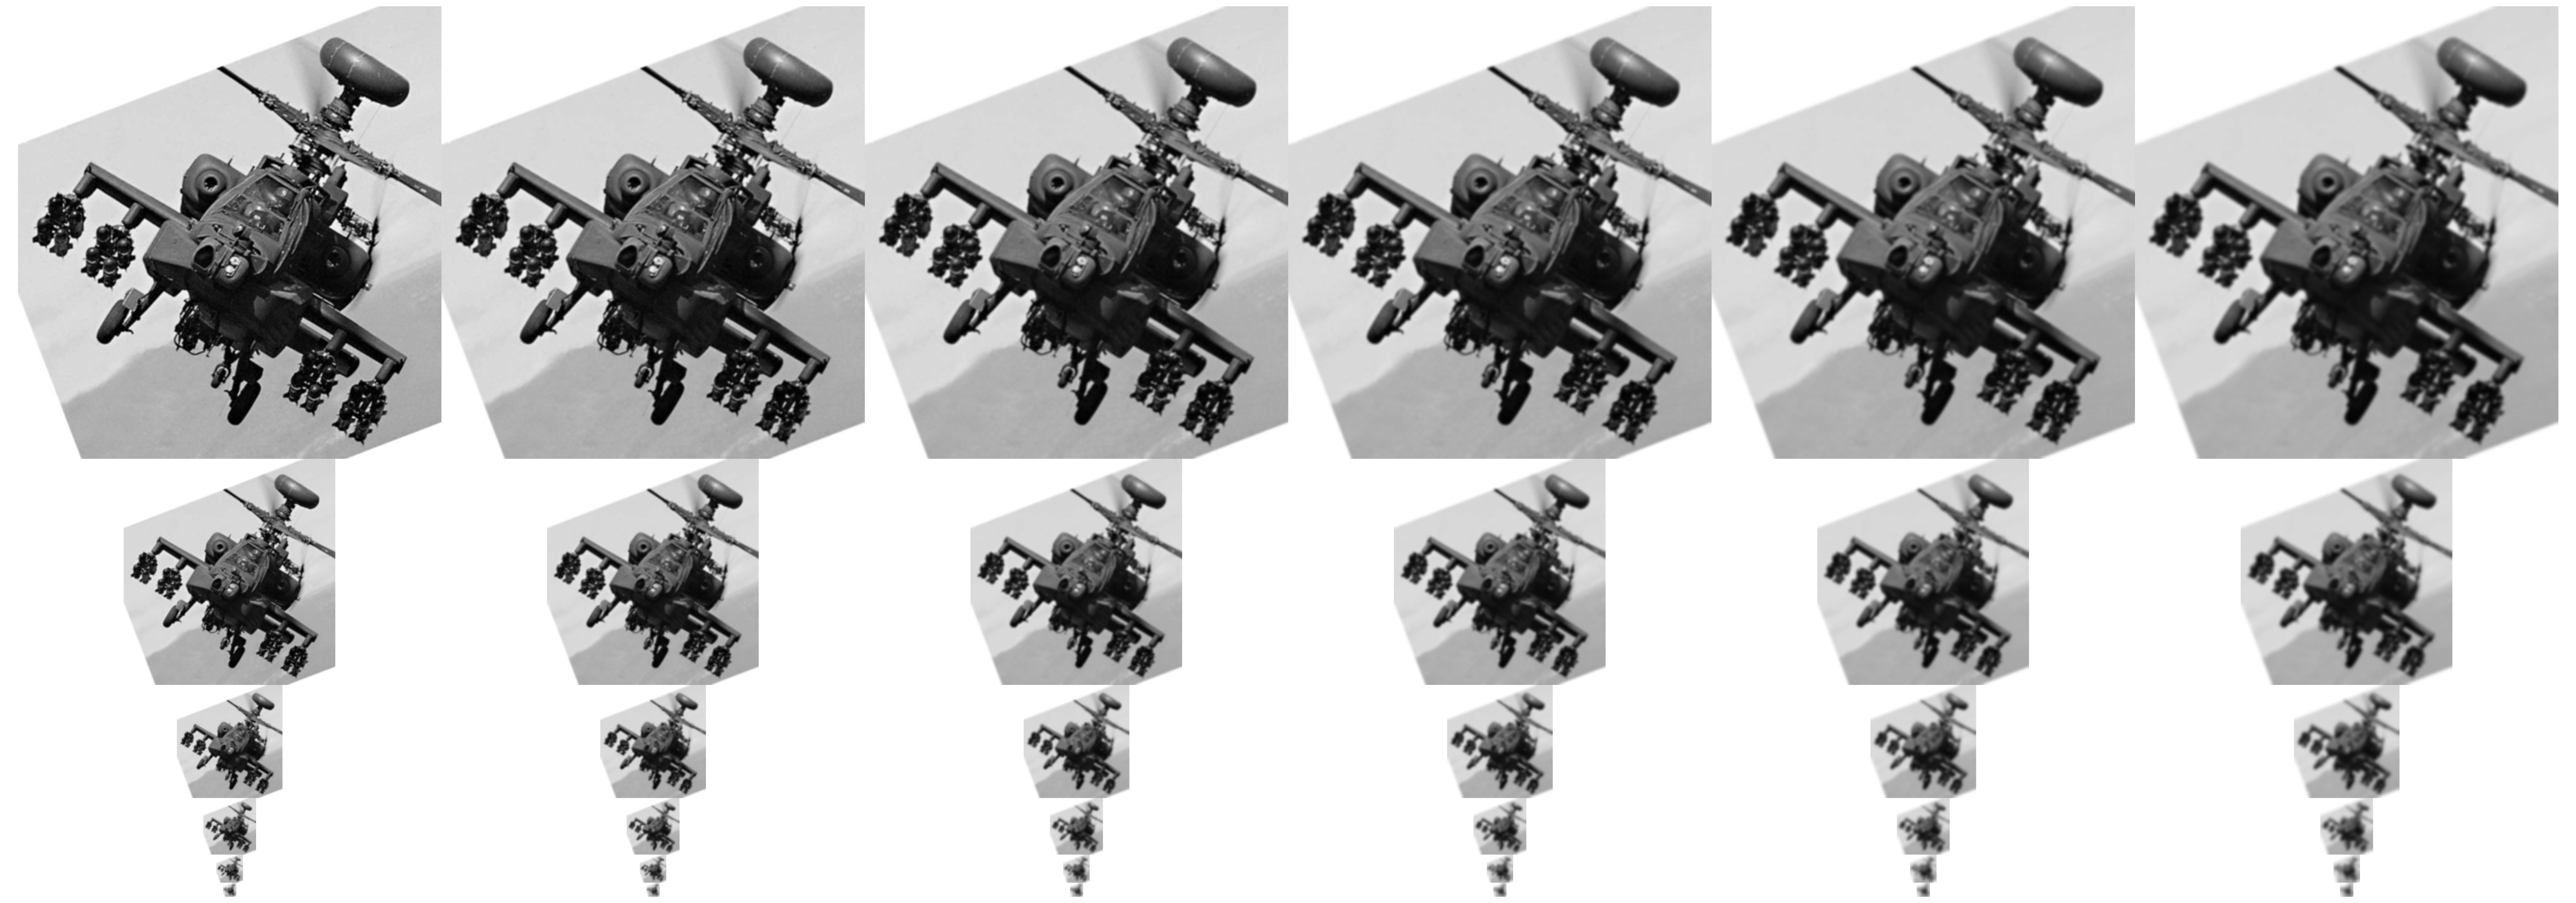
\includegraphics[width=1\textwidth]{./result/gauss_pyr}
\caption{高斯金字塔}
\end{figure}

\subsubsection{DoG金字塔}

    高斯金字塔中每组的相邻两层相减得到,高斯金字塔有每组\(S+3\)层图像。
    DoG金字塔每组有\(S+2\)层图像。得到的金字塔图像如图所示:
    由于后续使用中DoG金字塔的头尾两层不直接使用,
    仅用到中间的\(S\)层图像。这就解释了为什么开始需要\(S+3\)层图像。
    由于本次实验选取\(S = 3\),所以最开始为6层。

\begin{figure}[h]
\centering

\includegraphics[width=1\textwidth]{./result/DoG_pyr}
\caption{DoG金字塔}
\end{figure}

    这里图像极黑是合理的,因为高斯模糊得到的像素值差距并不大,
    需放大仔细看,能看到相对清晰的边缘。

\subsubsection{准确定位关键点}

    对于\( D(x, y, d) \)中的某个点,
    如果它的值大于或小于其周围的8个点和它上下相邻尺度的18个点,
    则该点是一个极值点。

\begin{figure}[h]
\centering
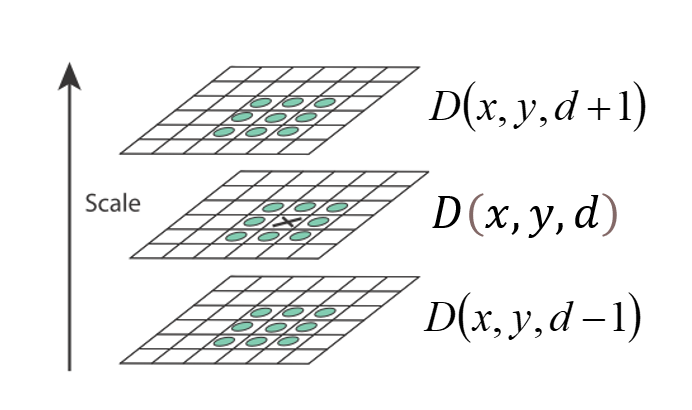
\includegraphics[width=0.8\textwidth]{./others/1}
\caption{原理图1}
\end{figure}

\newpage

    对于上述步骤中提取的尺度空间极值点,下一个步骤要对它们进行精选,
    排除掉一些低对比度的或位于边缘上的点。

    对函数\(D(x, y, d)\)做泰勒展开:

\[
    D(\vec{x}) = D(\vec{x_0})
    + \nabla D(\vec{x_0})^T (\vec{x} - \vec{x_0})
    + \frac{1}{2} (\vec{x} - \vec{x_0})^T \nabla^2 D(\vec{x_0}) (\vec{x} - \vec{x_0})
\]
    求导,令\(\nabla D(\vec{x}) = \vec{0}\)

    得

\[
    \hat{x} = -\left[\frac{\partial^2D}{\partial\vec{x}^2}\right]^{-1}\frac{\partial D}{\partial\vec{x}}
\]

\[
    D(X = \vec{x_0} + \hat{x}) = D(\vec{x_0}) + \frac{1}{2}\nabla D(\vec{x_0})^T \hat{x}
\]

    即经典的牛顿下降法。当\(\hat{x}\)中的每一个元素均处于\((-0.5, 0.5)\)范围内,就视为找到了极值点。
    根据论文,筛选出\(|D(X)| \geq 0.03\)的点作为特征点。(此处开始将像素值映射至\((0, 1)\)区间处理)

    另外,由于图像为离散的点,我们约定用以下方法求解梯度和Hessian矩阵

    对于梯度\(\nabla D(\vec{x})\), 我们选择其相邻的像素计算。
    考虑到间隔,我们将差值除以2。结果如下:

\[
    \nabla D(x, y, d) = \frac{1}{2}
    \begin{bmatrix}
        D(x, y + 1, d) - D(x, y - 1, d) \\
        D(x + 1, y, d) - D(x - 1, y, d) \\
        D(x, y, d + 1) - D(x, y, d - 1)
    \end{bmatrix}
\]
    这里方向看似有些奇怪,原因在于此处\(x, y\)按平面直角坐标系选取,
    而实际存储的\(x, y\)对应\(r, c\)。

    而对于Hessian矩阵,混合系数部分同理梯度算子,再次求导,
    用对应方向上的相邻像素点作差除2替代,最后带有常数\(\frac{1}{4}\).
    而主对角线上的三个元素,用以下方法,以x为例:

\[
    f''(x) = f'(x + 1) - f'(x) = f(x + 1) - f(x) - (f(x) - f(x - 1)
\]
\[
    f''(x) = f(x + 1) - 2f(x) + f(x - 1)
\]

    故不需要额外的系数。仿照上式计算即可。

    本次实验中采取迭代6次作为判断,如迭代6次仍不能稳定则舍去。
    同时对于Hessian矩阵不可逆的情况同样舍去。如迭代中遇到边界
    等情况同样舍去。

    论文中还提到要排除边缘处的关键点。具体方法如下:

    取Hessian矩阵左上角的\(2\times 2\)子矩阵H,记
\[
    H = \begin{bmatrix}
            H_{xx} & H_{xy} \\
            H_{yx} & H_{yy}
    \end{bmatrix}
\]

    矩阵的迹\(tr(H)\)和行列式\(det(H)\),如果

\[
    \frac{tr(H)^2}{det(H)} < \frac{(r_0 + 1)^2}{r_0}
\]
    则舍去这个关键点。论文取\(r_0 = 10\).

    其原因在于高斯函数的差值沿边缘有很强的响应,
    甚至会导致无法确定边缘,对少量噪声不稳定。
    (翻译自论文原文,但解释并不清晰,参考其4.1节)

\begin{figure}[h]
\centering
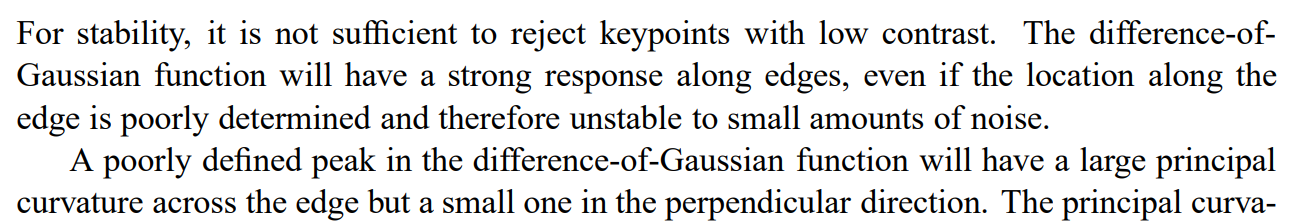
\includegraphics[width=1\textwidth]{./others/a2}
\caption{论文原文2}
\end{figure}

    而在实验中发现单纯按上述方法提取关键点存在问题。
    仅根据DoG图中的数值为周围像素点极值提取的像素点这一限制条件,
    会提取多达2e6以上数量的潜在特征点。其远远超出了计算机的处理能力。
    原因在于多数空间范围由于像素变化不大,整体差值接近0导致的。
    这显然不是我们希望的特征点。故在第一步筛选时增加了DoG绝对值
    大于等于0.04和0.03两组限制条件,期望得到更好的边缘点
    并减小后续计算复杂度。在上述限制条件下,潜在特征点的数量分别
    降至2405和4756,特征点数量降至866和1605,具体结果如下图所示(左图为0.04,右图为0.03):

\newpage

\begin{figure}[h]
\centering
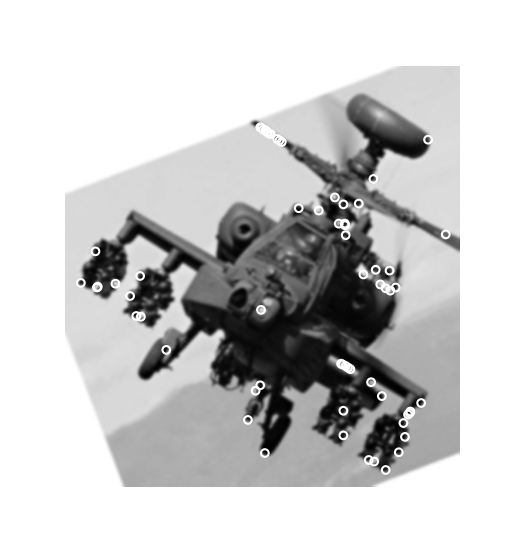
\includegraphics[width=0.4\textwidth]{./result/004}
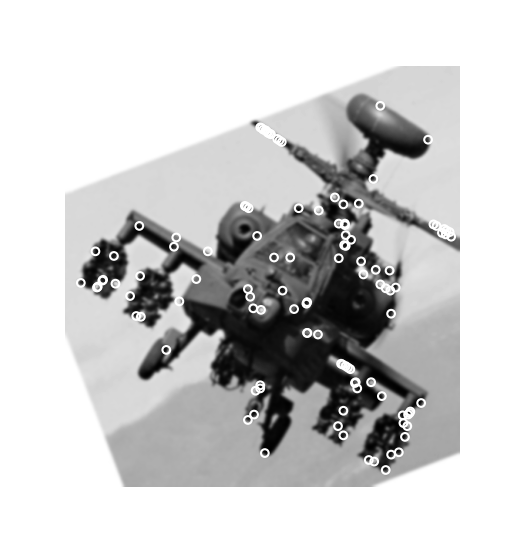
\includegraphics[width=0.4\textwidth]{./result/003}
\caption{特征点提取结果}
\end{figure}

\begin{figure}[h]
\centering
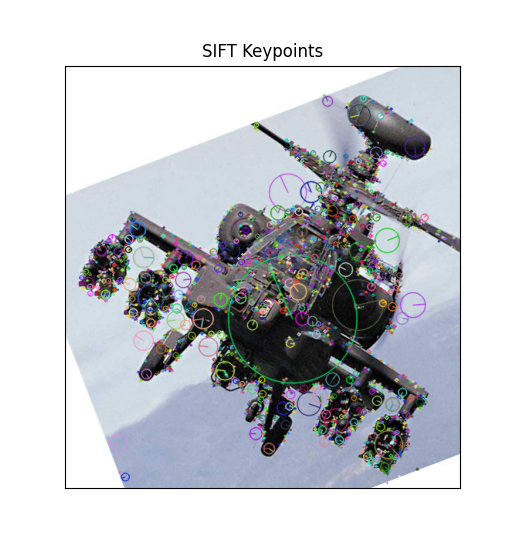
\includegraphics[width=0.4\textwidth]{./result/standard}
\caption{标准库结果}
\end{figure}

    对比标准库结果可以发现,0.03组效果接近标准库的实现,但仍然
    存在特征提取不足,部分区域特征提取过密等情况。同时,标准库的
    运行时间远小于手动实现的特征点提取。因此后续实验采用opencv
    标准库的goodFeaturesToTrack函数实现特征提取(即Harris
    方法)
    
\subsection{图像关键点提取——Harris角点提取函数}

    与用高斯差分构建的尺度空间不同,
    图像金字塔通过直接缩放图像的方式构建尺度空间。

    通过 im2 = cv2.resize(im1,(size,size))函数
    可以快速构建一系列分辨率不一的图像,再通过对应函数提取角点。

    主要用到cv2.goodFeaturesToTrack(image, maxCorners, qualityLevel, minDistance
    [,corners[,mask[,blockSize[,useHarrisDetector[,k]]]]])->corners

    image:输入图像;

    maxCorners:允许返回的最多角点个数,设为200;

    qualityLevel: 图像角点的最小可接受参数,
    质量测量值乘以这个参数就是最小特征值,小于这个数的会被抛弃,设为0.01;

    minDistance: 返回的角点之间最小的欧式距离, 设为10;

    blockSize:邻域大小,设为3;

    k:Harris检测的自由参数,越小返回的角点数越多,设为0.04。\\

    检测结果如图所示:

\begin{figure}[h]
\centering
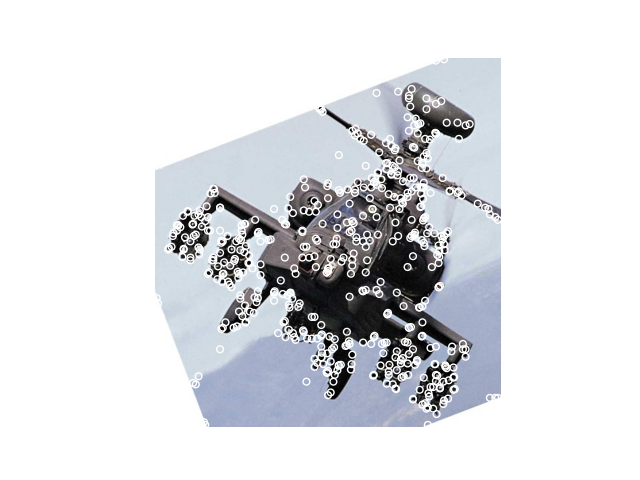
\includegraphics[width=0.4\textwidth]{./result/findcorner}
\caption{Harris角点检测结果}
\end{figure}

\subsection{SIFT描述子}

    SIFT描述子之所以具有旋转不变的性质是因为
    人们能通过物体的局部细节潜在地建立起物体坐标系,
    并建立其和图像坐标系之间的映射关系。而物体之间的相对
    关系并不随图像的旋转发生变化。

    SIFT描述子把以关键点为中心的邻域内的主要梯度方向
    作为物体坐标系的X方向,因为该坐标系是由关键点本身的性质定义的,
    因此具有旋转不变性。

    对应论文第5节:假设某尺度下某关键点为L(x, y),
    对于它m*m邻域内(其所在高斯金字塔图像3σ邻域窗口内)的每个点,
    计算其在该尺度下的梯度强度和梯度方向(这里无需缩放,因为比例因子的贡献会抵消):

\[
    mag(x, y) = \sqrt{\left(L(x + 1, y) - L(x - 1, y)\right)^2 + \left(L(x, y + 1) - L(x, y - 1)\right)^2}
\]

\[
    \theta(x, y) = tan^{-1}\left[\frac{L(x, y + 1) - L(x, y - 1)}{L(x + 1, y) - L(x - 1, y)}\right]
\]

    随后根据\(\theta\)的值(需根据\(L_x, L_y\)的正负确定方向,范围为\([0, 360)\))
    分成36等分,将梯度强度乘上该点对应的高斯函数值(作为权重)加入对应方向,
    以类似于直方图的形式统计。

    实验中简化了论文的做法,只选取了最大的方向作为SIFT算子的方向,即物体坐标系的x轴正方向。
    逆时针旋转90°得y轴正方向。

    再根据对应的x,y轴方向,选取\(16 \times 16\)个像素,分成\(4 \times 4\)组,每组\(4 \times 4\)个像素。
    对于每组,将梯度强度按梯度方向统计至对应的八个方向,这样一共有\(16 \times 8\)个方向,归一化
    (除以平方和的平方根,L2-norm)后即SIFT特征值。

    对于最后的匹配,暴力枚举两张图片中的关键点,选择SIFT特征值点积最大且大于0.7的组,认为它们是匹配的关键点。

    以上为理论分析。在实际代码中做了以下的调整:

    1.考虑到\(3\sigma\)范围的像素点选取和图像降采样导致的等效\(\sigma\)减半,对每张图像做一次高斯模糊,使其
    \(\sigma = 1.6\)

    2.根据论文内容,这边选择了半径为\(3\times 1.5\times \sigma\)作为实际统计的范围。代码中为避免麻烦统计了
    正方形区域,理论而言如果选择圆形区域效果会更好。

\begin{figure}[h]
\centering
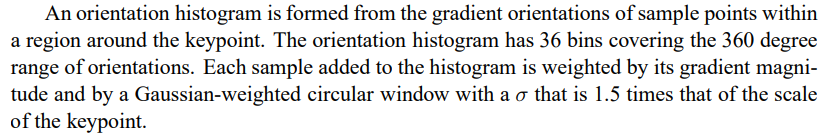
\includegraphics[width=1\textwidth]{./others/a3}
\caption{论文原文3}
\end{figure}

    3.考虑低分辨率图像的范围不足,代码中选择求得梯度方向后映射至原始图像求解SIFT特征值。
    也可以尝试直接在对应图像上进行求解。由于未做对比实验,无法确定两者做法的优劣。

    4.对于SIFT特征值的计算:由于像素为离散值,这里选择了中心坐标\(\pm7.5\),间隔为1的方式选取了256个像素点。
    根据得到的\(\theta\)值,对相对坐标做变换

\[
    rotary = \begin{bmatrix}
                 cos(\theta) & -sin(\theta) \\
                 sin(\theta) & cos(\theta)
    \end{bmatrix}
\]
    加上中心点坐标得到对应坐标。首先对四个角进行检测,如存在超出边界的则舍去这个点。
    随后进行相应的统计即可。如果求得的像素不为整点,使用双线性插值方法,以周围四个整点的
    梯度值插值得该像素的梯度大小及方向。如图所示:

\begin{figure}[h]
\centering
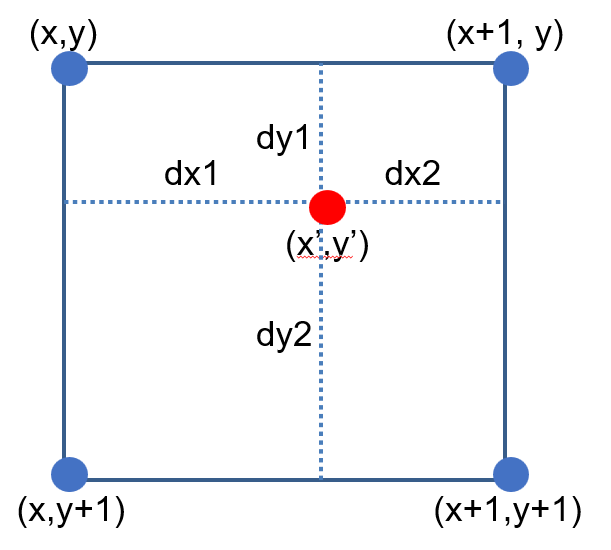
\includegraphics[width=0.4\textwidth]{./others/2}
\caption{双线性插值}
\end{figure}

\section{代码运行结果}

\subsection{手动实现的结果}

\begin{figure}[h]
\centering
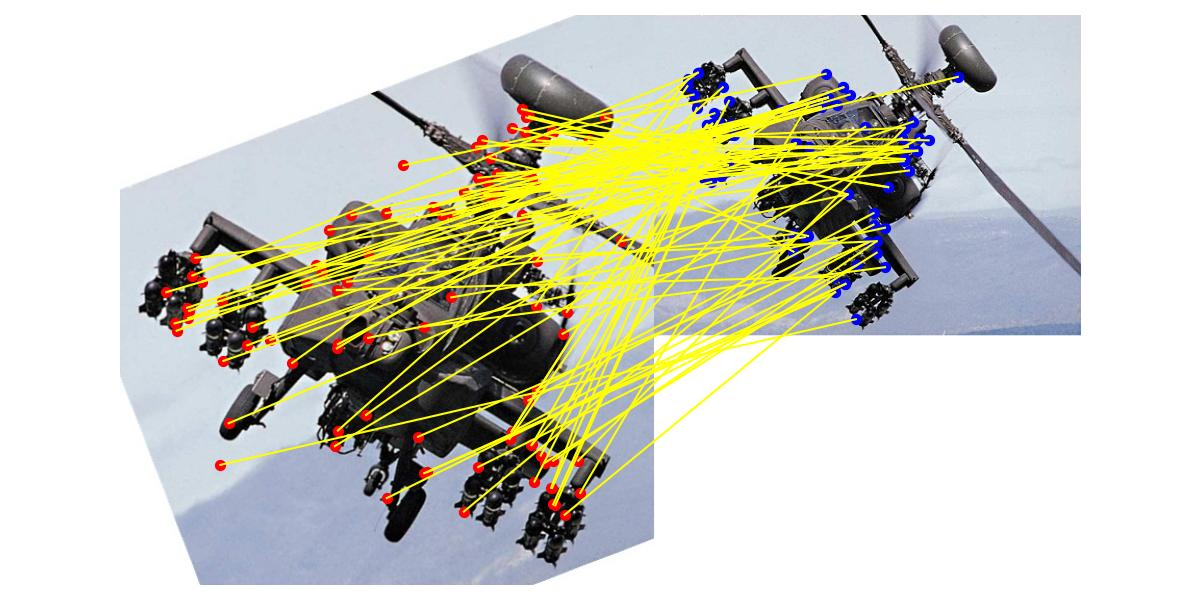
\includegraphics[width=0.6\textwidth]{./result/3}
\caption{匹配结果1}
\end{figure}

    通过比较生成的特征点数量,代码能正确找到匹配最多的图像。
    但由于部分实现的简化和参数设置问题,匹配未能实现理想情况下
    关键点连线基本平行的结果。

    其原因可能在于局部特征的相似性导致相对位置不同的点被误认为匹配,
    如飞机下端对称的发射器。也有可能是代码中对于高维特征提取不足导致的。

\begin{figure}[h]
\centering
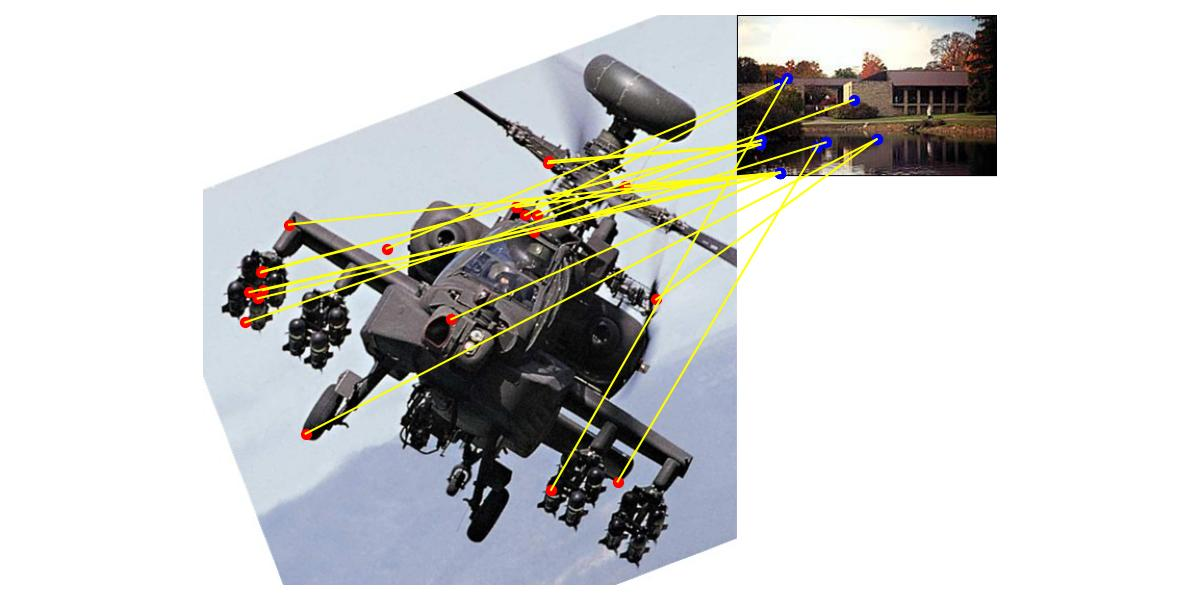
\includegraphics[width=0.4\textwidth]{./result/1}
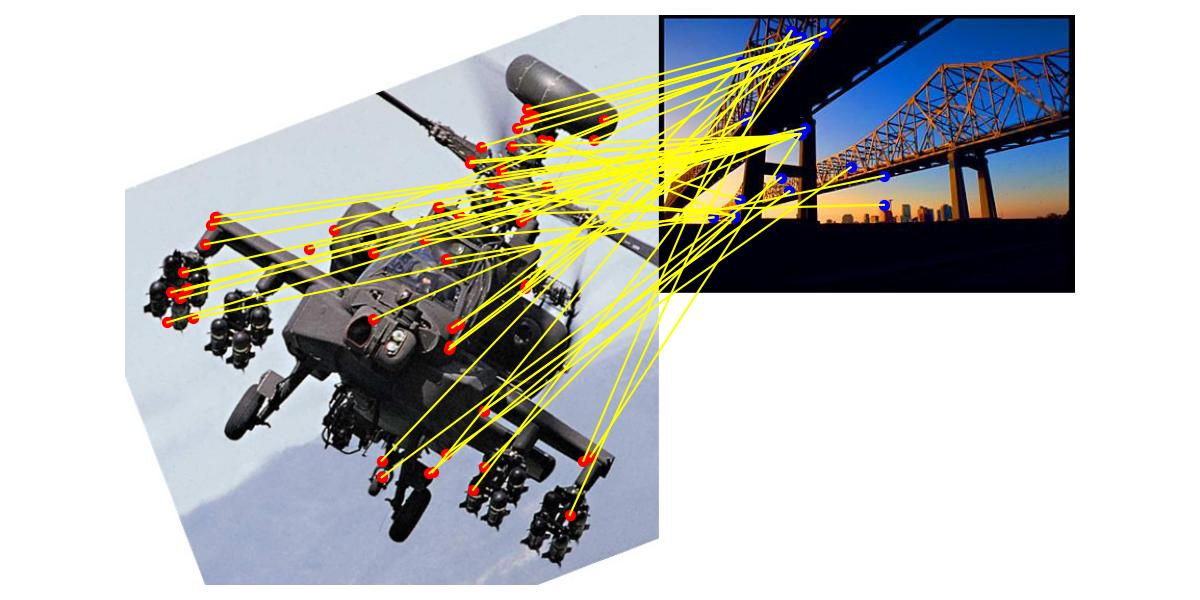
\includegraphics[width=0.4\textwidth]{./result/2}
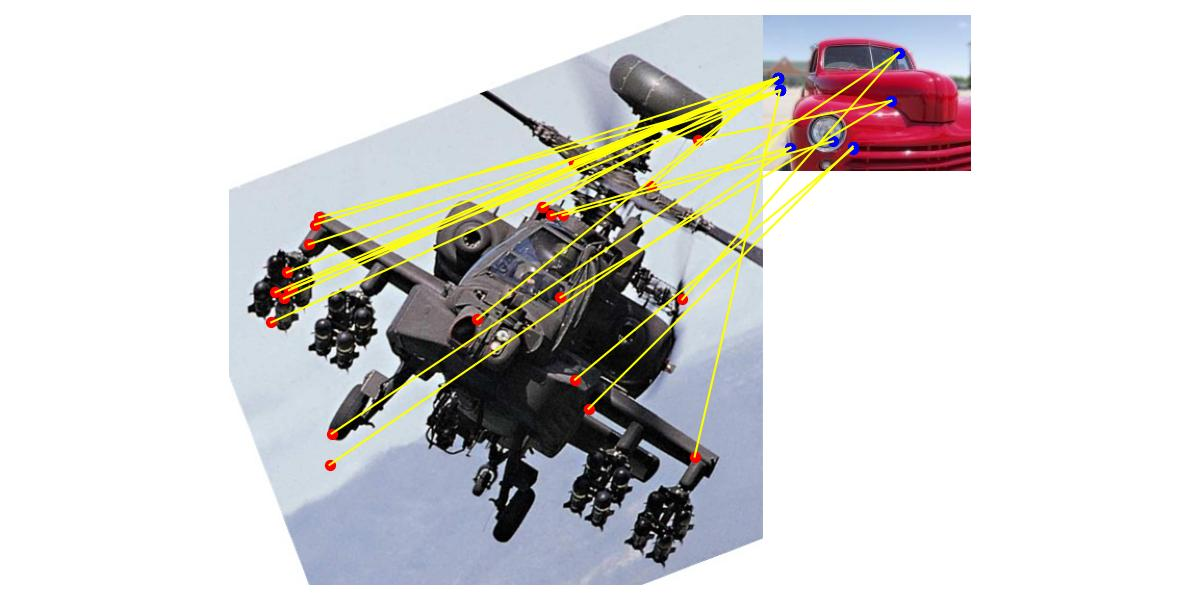
\includegraphics[width=0.4\textwidth]{./result/4}
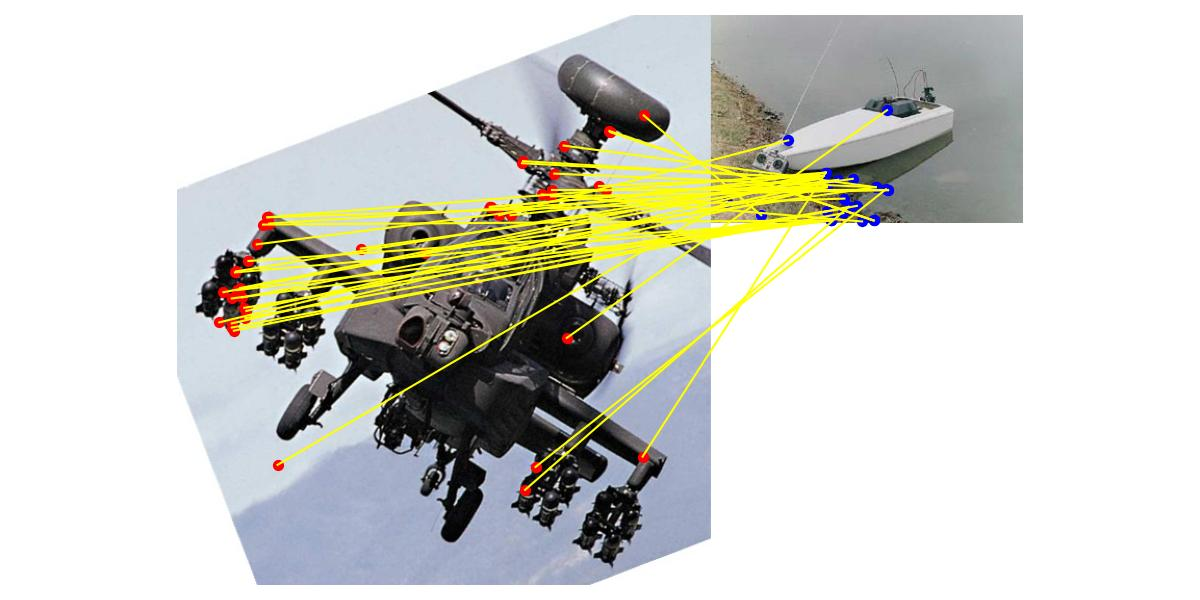
\includegraphics[width=0.4\textwidth]{./result/5}
\caption{匹配结果2}
\end{figure}

    以上依次为图1、2、4、5的匹配结果。图2中特征点匹配数量较多,
    可能是由于桥身主体为黑色,接近飞机特征所致。

\subsection{系统库的实现结果}
\newpage

\begin{figure}[h]
\centering
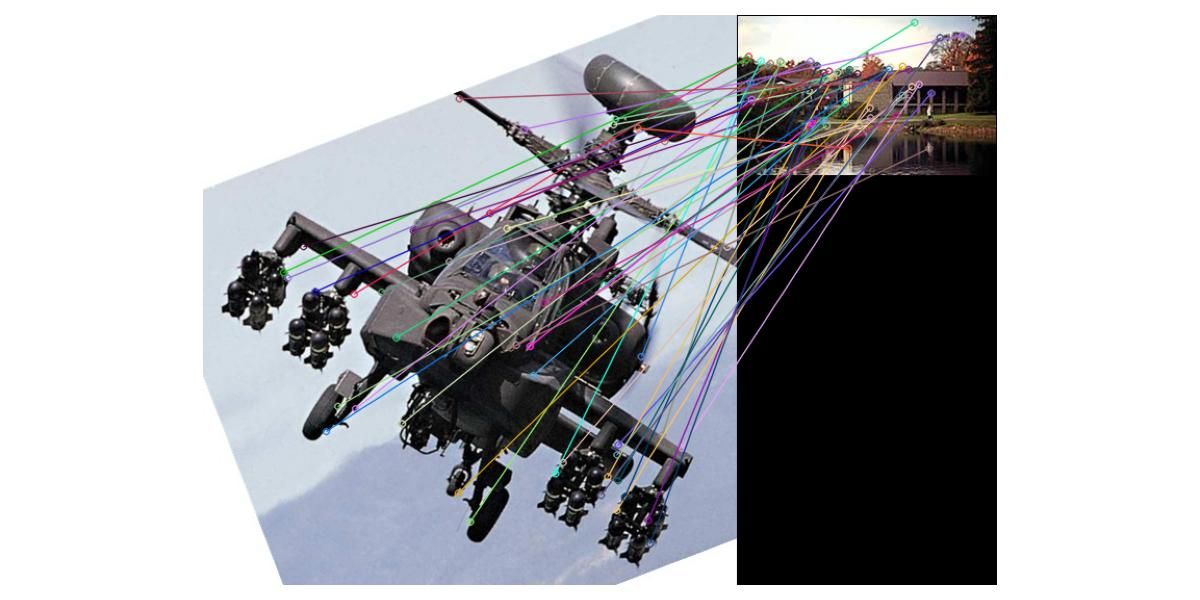
\includegraphics[width=0.4\textwidth]{./official/1}
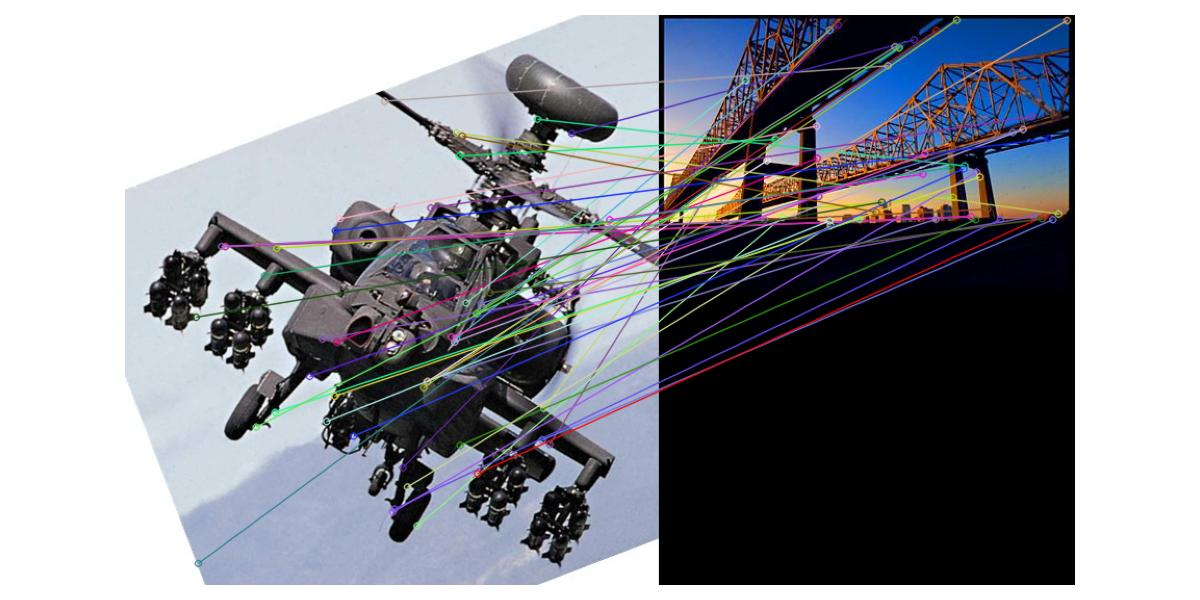
\includegraphics[width=0.4\textwidth]{./official/2}
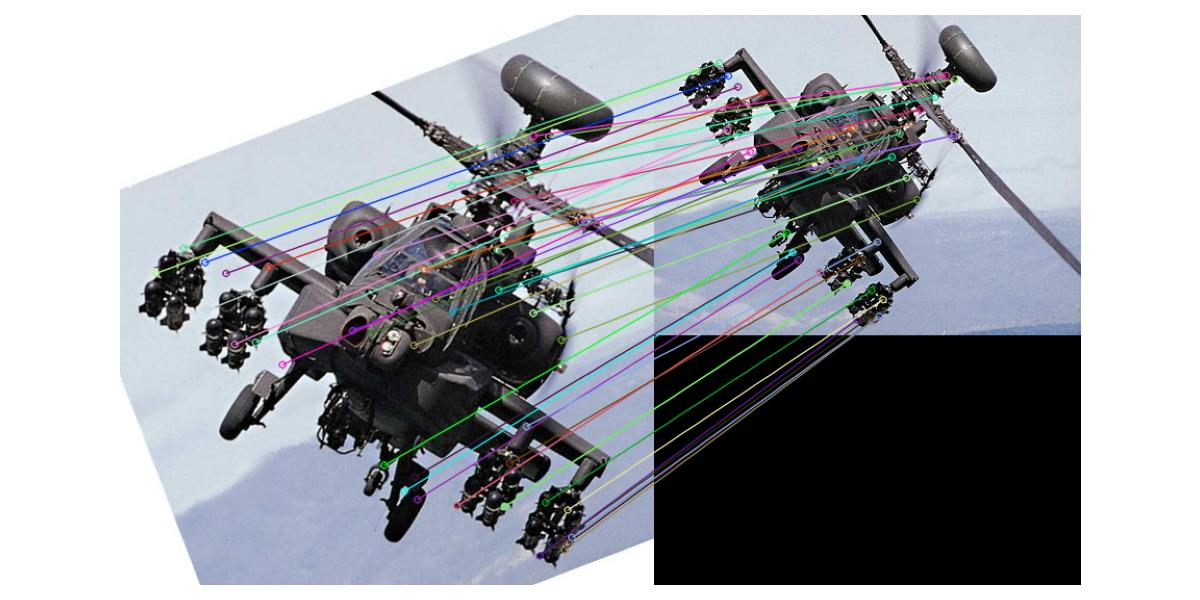
\includegraphics[width=0.6\textwidth]{./official/3}
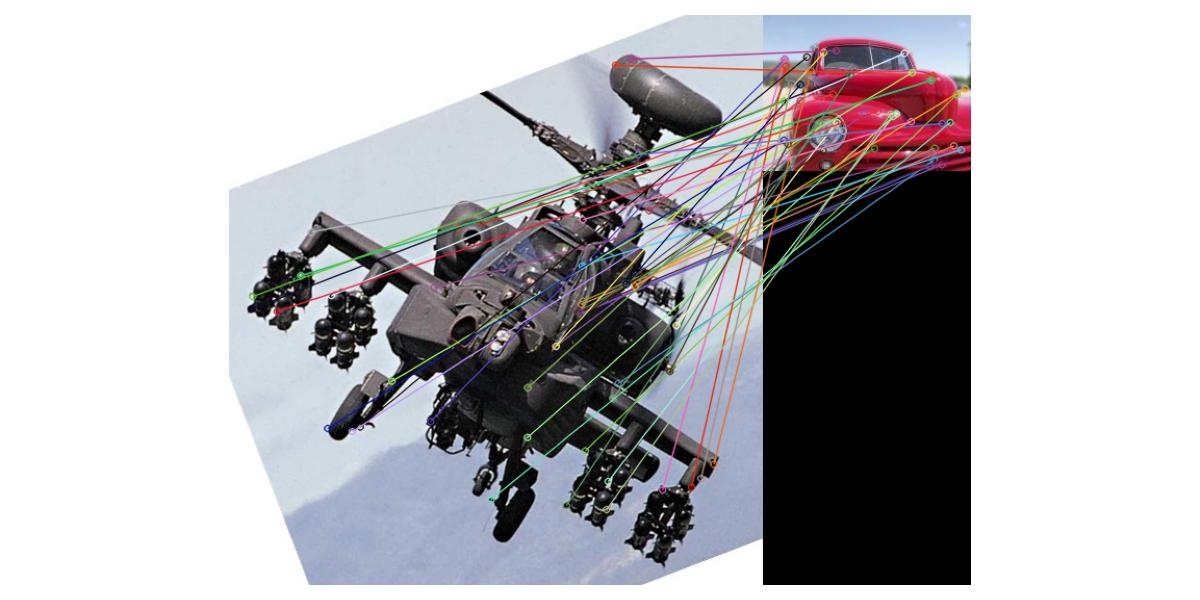
\includegraphics[width=0.4\textwidth]{./official/4}
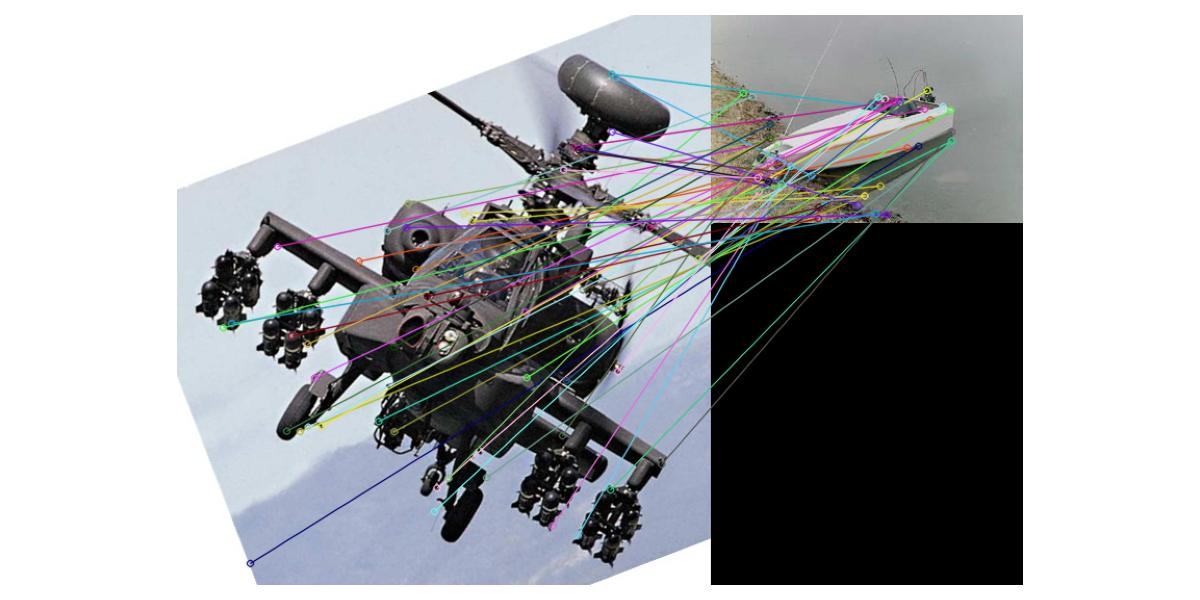
\includegraphics[width=0.4\textwidth]{./official/5}
\caption{匹配结果3}
\end{figure}

    对于正确的匹配(图3)系统库的关键点匹配效果远好于手动实现,
    且速度较快(1s,手动实现计算五幅图共用时30s左右)总体而言,
    手动实现的代码仍有很多地方可以改进。

\section{实验感想}

    本次实验学习了SIFT算法的实现,对于图像识别算法有了更深入的认识。
    高斯模糊和高斯差分是有效的图像特征提取的手段,在神经网络尚未发展
    的过去,这一系列传统方法的实现思路对当今图像识别和计算机视觉的发展
    仍然有参考价值。

\section{相关实现代码}

\subsection{高斯金字塔方法提取特征点:gauss\_method.py}


\begin{lstlisting}
    import cv2
import numpy as np
import matplotlib.pyplot as plt
import math

from numpy import dtype
from scipy.ndimage import zoom

image = cv2.imread('./target.jpg', cv2.IMREAD_GRAYSCALE)
H, W = image.shape

def gauss_filter(sigma=1.6, k = 3):
    ax = np.arange(-k, k + 1)
    x, y = np.meshgrid(ax, ax)
    gauss_mat = np.exp(-(x ** 2 + y ** 2) / (2 * sigma ** 2))
    gauss_mat /= 2 * np.pi * sigma ** 2
    return gauss_mat / gauss_mat.sum()

nOctaves = math.floor(math.log2(min(W, H))) - 3
nOctaveLayers = 3
k = 2 ** (1 / nOctaveLayers)
sigma0 = 1.6

scale = 2
image = zoom(image, scale, order=3)

sigma_init = (sigma0 ** 2 - (2 * 0.5) ** 2) ** 0.5
gauss_core = gauss_filter(sigma_init)
image = cv2.filter2D(image, -1, gauss_core)

gauss_pyr_img = [None] * nOctaves
DoG_pyr_img = [None] * nOctaves
img_i = image

for i in range(nOctaves):
    gauss_oct_i = np.zeros((nOctaveLayers + 3, img_i.shape[0], img_i.shape[1]), dtype = img_i.dtype)
    gauss_oct_i[0, :, :] = np.copy(img_i)
    for j in range(1, nOctaveLayers + 3):
        sigma_pre = k ** (j - 1) * sigma0
        sigma_dif = ((k * sigma_pre) ** 2 - sigma_pre ** 2) ** 0.5
        G_C = gauss_filter(sigma_dif)
        img_i = cv2.filter2D(img_i, -1, G_C)
        gauss_oct_i[j, :, :] = np.copy(img_i)
    gauss_pyr_img[i] = np.copy(gauss_oct_i)
    DoG_pyr_img[i] = np.copy(gauss_oct_i.astype(np.int32)[1:, :, :] - gauss_oct_i.astype(np.int32)[:-1, :, :]).astype(np.int32)
    img_i = zoom(gauss_oct_i[-3, :, :], 0.5, order = 3)

# max_width = max([sum(img.shape[1] for img in group) for group in DoG_pyr_img])
# total_height = sum(group[0].shape[0] for group in DoG_pyr_img)
#
# canvas = np.ones((total_height, max_width)) * 255

# y_offset = 0
# for group in DoG_pyr_img:
#     group_height = group[0].shape[0]
#     x_offset = int(W - group[0].shape[1] / 2)
#     for img in group:
#         h, w = img.shape
#         canvas[y_offset:y_offset + h, x_offset:x_offset + w] = img
#         x_offset += W * 2
#     y_offset += group_height
#
#
# plt.figure(figsize=(max_width / 100, total_height / 100))
# plt.imshow(canvas, cmap='gray')
# plt.axis('off')
# plt.tight_layout()
# plt.savefig("./result/DoG_pyr1.png")

ext = []
min_val = 0.03 * 255
for i in range(nOctaves):
    DoG = DoG_pyr_img[i]
    num, h, w = DoG.shape
    for j in range(1, num - 1):
        for r in range(4, h - 3):
            for c in range(4, w - 3):
                neigh = np.copy(DoG[j - 1: j + 2, r - 1: r + 2, c - 1: c + 2])
                val = neigh[1][1][1]
                if abs(val) > min_val and (val == np.max(neigh) or val == np.min(neigh)):
                    sigma_i = k ** j * sigma0
                    ext.append([i, j, r, c, sigma_i])
keypoint = []
for i in range(len(ext)):
    kpt = ext[i]
    num_oct = kpt[0]
    num_lay = kpt[1]
    r = kpt[2]
    c = kpt[3]
    should_delete = True
    D_hat = None

    for iter in range(6):
        DoG = DoG_pyr_img[num_oct][num_lay] / 255
        DoG_pre = DoG_pyr_img[num_oct][num_lay - 1] / 255
        DoG_nxt = DoG_pyr_img[num_oct][num_lay + 1] / 255

        dD = np.array([[DoG[r, c + 1] - DoG[r, c - 1]],
                       [DoG[r + 1, c] - DoG[r - 1, c]],
                       [DoG_pre[r, c] - DoG_nxt[r, c]]
                      ]) / 2
        dxx = (DoG[r, c + 1] + DoG[r, c - 1] - 2 * DoG[r, c]) / 1
        dyy = (DoG[r + 1, c] + DoG[r - 1, c] - 2 * DoG[r, c]) / 1
        dss = (DoG_pre[r, c] + DoG_nxt[r, c] - 2 * DoG[r, c]) / 1

        dxy = (DoG[r + 1, c + 1] + DoG[r - 1, c - 1] - DoG[r + 1, c - 1] - DoG[r - 1, c + 1]) / 4
        dxs = (DoG_nxt[r, c + 1] - DoG_nxt[r, c - 1] - DoG_pre[r, c + 1] + DoG_pre[r, c - 1]) / 4
        dys = (DoG_nxt[r + 1, c] - DoG_nxt[r - 1, c] - DoG_pre[r + 1, c] + DoG_pre[r - 1, c]) / 4

        dH = np.array([[dxx, dxy, dxs], [dxy, dyy, dys], [dxs, dys, dss]])
        if np.linalg.det(dH) == 0:
            break
        x_hat = np.linalg.inv(dH) @ dD

        if abs(x_hat[0][0]) < 0.5 and abs(x_hat[1][0]) < 0.5 and abs(x_hat[2][0]) < 0.5:
            should_delete = False
            break

        c = c + round(x_hat[0][0])
        r = r + round(x_hat[1][0])
        num_lay = num_lay + round(x_hat[2][0])

        if  num_lay < 1 or num_lay > nOctaveLayers or \
            r <= 0 or r >= DoG_pyr_img[num_oct][num_lay].shape[0] - 1 or \
            c <= 0 or c >= DoG_pyr_img[num_oct][num_lay].shape[1] - 1:
            break


    if should_delete:
        continue

    D_hat = DoG[r][c] + (dD.T @ x_hat) / 2
    if abs(D_hat) < 0.03:
        continue

    trH = dxx + dyy
    detH = dxx * dyy - dxy * dxy
    r0 = 10

    if detH <= 0 or trH * trH * r0 >= (r0 + 1) * (r0 + 1) * detH:
        continue

    keypoint.append([num_oct, num_lay, r, c, k**num_lay * sigma0])

H, W = gauss_pyr_img[1][1].shape

fig, ax = plt.subplots(figsize=(W / 100, H / 100), dpi=100)

ax.imshow(gauss_pyr_img[1][1], cmap='gray')
ax.axis("off")

ax.set_xlim(0, W)
ax.set_ylim(0, H)
ax.invert_yaxis()

for i in range(len(keypoint)):
    kpt = keypoint[i]
    num_oct = kpt[0]
    num_lay = kpt[1]
    if num_oct == 1 and num_lay == 1:
        r = kpt[2]
        c = kpt[3]
        if 0 <= r < H and 0 <= c < W:
            circle = plt.Circle((c, r), radius=5, color='white', fill=False, linewidth=1.5)
            ax.add_patch(circle)

plt.show()
plt.close()
\end{lstlisting}

\subsection{Harris算法和SIFT特征值求解及匹配:main.py}

\begin{lstlisting}
    import cv2
import numpy as np
import matplotlib.pyplot as plt
import math


def gauss_filter(sigma=1.6, k = 3):
    ax = np.arange(-k, k + 1)
    x, y = np.meshgrid(ax, ax)
    gauss_mat = np.exp(-(x ** 2 + y ** 2) / (2 * sigma ** 2))
    gauss_mat /= 2 * np.pi * sigma ** 2
    return gauss_mat / gauss_mat.sum()

def rotary_matrix(theta):
    rad = theta / 180 * math.pi
    return np.array([[math.cos(rad), -math.sin(rad)], [math.sin(rad), math.cos(rad)]])

def sift_opt(path):
    image = cv2.imread(path, cv2.IMREAD_COLOR)
    image_grey = cv2.cvtColor(image, cv2.COLOR_BGR2GRAY)
    H, W = image_grey.shape

    img = []
    sigma = 1.6
    init_image = cv2.filter2D(image_grey, -1, gauss_filter(sigma = (sigma ** 2 - 0.5 * 0.5) ** 0.5))
    img.append(init_image)

    scale = 2
    level = math.floor(math.log2(min(H, W))) - 3
    for i in range(level):
        prev_img = img[-1]
        new_width = prev_img.shape[1] // scale
        new_height = prev_img.shape[0] // scale
        img1 = cv2.resize(prev_img, (new_width, new_height))
        img1 = cv2.filter2D(img1, -1, gauss_filter(sigma = (sigma ** 2 - (0.5 * sigma) ** 2) ** 0.5))
        img.append(img1)

    keypoints = []
    for i, imgi in enumerate(img):
        corners = cv2.goodFeaturesToTrack(imgi, maxCorners=300, qualityLevel=0.01, minDistance=8, blockSize=3, k=0.04)
        for j in corners:
            keypoints.append(np.array([j[0][0], j[0][1], i]))

    filter = []
    for kpt in keypoints:
        x = int(kpt[0])
        y = int(kpt[1])
        layer = int(kpt[2])
        radius = round(3 * 1.5 * sigma)
        img_i = img[layer]
        h, w = img_i.shape


        deg = np.zeros(36, dtype = int)
        for i in range(-radius, radius + 1):
            r = x + i
            if r <= 0 or r >= h - 1:
                continue
            for j in range(-radius, radius + 1):
                c = y + j
                if c <= 0 or c >= w - 1:
                    continue
                dx = int(img_i[r][c + 1]) - int(img_i[r][c - 1]) / 2
                dy = int(img_i[r - 1][c]) - int(img_i[r + 1][c]) / 2

                dx = int(dx)
                dy = int(dy)

                mag = (dx * dx + dy * dy) ** 0.5
                if dy >= 0:
                    ang = math.atan2(dy, dx)
                else:
                    ang = math.atan2(dy, dx) + 2 * math.pi
                ang = ang * 180 / math.pi

                bin = round(0.1 * ang)
                if bin >= 36:
                    bin -= 36
                elif bin < 0:
                    bin += 36
                weight = np.exp(-(i ** 2 + j ** 2) /  (2 * radius ** 2))
                deg[bin] += mag * weight
        is_zero = True
        for i in range(len(deg)):
            if deg[i] != 0:
                is_zero = False
        if is_zero:
            continue
        max_deg = max(deg)
        for i in range(36):
            if deg[i] == max_deg:
                dir = i
        filter.append((x * (2 ** (layer)), y * (2 ** (layer)), dir))



    sift = []
    for i in range(len(filter)):
        is_edge = False
        x = filter[i][0]
        y = filter[i][1]
        theta = filter[i][2] * 10
        for j in (-7.5, 7.5):
            for k in (-7.5, 7.5):
                R_M = rotary_matrix(theta)
                pos = R_M @ np.array([[j], [k]])
                x_ = pos[0][0] + x
                y_ = pos[1][0] + y
                if x_ <= 2 or x_ >= H - 3 or y_ <= 2 or y_ >= W - 3:
                    is_edge = True
        if is_edge:
            continue

        cnt = np.zeros((4, 4, 8), dtype = float)
        for j in range(-8, 8):
            for k in range(-8, 8):
                R_M = rotary_matrix(theta)
                pos = R_M @ np.array([[j + 0.5], [k + 0.5]])
                x_ = pos[0][0] + x
                y_ = pos[1][0] + y

                dx1 = x_ - math.floor(x_)
                dx2 = math.ceil(x_) - x_
                dy1 = y_ - math.floor(y_)
                dy2 = math.ceil(y_) - y_

                _x = math.floor(x_)
                _y = math.floor(y_)

                gradxy = np.array([int(image_grey[_x][_y + 1]) - int(image_grey[_x][_y - 1]),
                                   int(image_grey[_x - 1][_y]) - int(image_grey[_x + 1][_y])]) / 2
                gradx1y1 = np.array([int(image_grey[_x + 1][_y + 2]) - int(image_grey[_x + 1][_y]),
                                    int(image_grey[_x][_y + 1]) - int(image_grey[_x + 2][_y + 1])]) / 2
                gradx1y = np.array([int(image_grey[_x + 1][_y + 1]) - int(image_grey[_x + 1][_y]),
                                   int(image_grey[_x][_y]) - int(image_grey[_x + 2][_y])]) / 2
                gradxy1 = np.array([int(image_grey[_x][_y + 2]) - int(image_grey[_x][_y]),
                                   int(image_grey[_x - 1][_y + 1]) - int(image_grey[_x + 1][_y + 1])]) / 2

                dxy = dx2 * dy2 * gradxy + dx1 * dy1 * gradx1y1 + dx1 * dy2 * gradx1y + dx2 * dy1 * gradxy1
                DX = dxy[0]
                DY = dxy[1]

                mag = (DX * DX + DY * DY) ** 0.5
                if DY >= 0:
                    ang = math.atan2(DY, DX)
                else:
                    ang = math.atan2(DY, DX) + 2 * math.pi
                ang = ang * 180 / math.pi

                bin = round(ang / 45)
                if bin >= 8:
                    bin -= 8
                elif bin <0:
                    bin += 8
                posi = math.floor((j + 8) / 4)
                posj = math.floor((k + 8) / 4)
                cnt[posi][posj][bin] += mag
        is_empty = True
        for _ in cnt:
            for __ in _:
                for ___ in __:
                    if ___ != 0:
                        is_empty = False
        if is_empty:
            continue
        cnt = cnt / (np.sum(np.square(cnt)) ** 0.5)
        cnt = cnt.reshape(1, -1)
        sift.append((x, y, np.copy(cnt)))
    return sift

path1 = "./target.jpg"

sift1 = sift_opt(path1)
for idx in range(1, 6):
    path2 = "./dataset/"+str(idx)+".jpg"
    sift2 = sift_opt(path2)

    num = 0
    match = []
    for i in range(len(sift1)):
        maxn = 0.0
        id = 0
        for j in range(len(sift2)):
            tot = 0.0
            for k in range(128):
                tot += sift1[i][2][0][k] * sift2[j][2][0][k]
            if tot > maxn:
                maxn = tot
                id = j
        if maxn >= 0.7:
            match.append((i, id))
            # num += 1

    img1 = cv2.imread(path1, cv2.IMREAD_COLOR)
    img2 = cv2.imread(path2, cv2.IMREAD_COLOR)

    img1 = cv2.cvtColor(img1, cv2.COLOR_BGR2RGB)
    img2 = cv2.cvtColor(img2, cv2.COLOR_BGR2RGB)

    h1, w1, _ = img1.shape
    h2, w2, _ = img2.shape

    canvas_height = max(h1, h2)
    canvas_width = w1 + w2
    canvas = 255 * np.ones((canvas_height, canvas_width, 3), dtype=np.uint8)

    canvas[:h1, :w1, :] = img1
    canvas[:h2, w1:w1 + w2, :] = img2

    plt.figure(figsize=(12, 6))
    plt.imshow(canvas)
    for (i, j) in match:

        x1 = sift1[i][0]
        y1 = sift1[i][1]

        x2 = sift2[j][0]
        y2 = sift2[j][1]

        plt.scatter(x1, y1, color='red', s=50)
        plt.scatter(x2 + w1, y2, color='blue', s=50)

        plt.plot([x1, x2 + w1], [y1, y2], color='yellow', linewidth=1.5)

    plt.axis('off')
    plt.tight_layout()
    plt.savefig("./result/"+str(idx)+".jpg")

    plt.close()
\end{lstlisting}

\subsection{官方库实现:official.py}
\begin{lstlisting}
    import cv2
import matplotlib.pyplot as plt
import math
import numpy as np

target_image_path = './target.jpg'
dataset_image_paths = ['./dataset/1.jpg', './dataset/2.jpg', './dataset/3.jpg', './dataset/4.jpg', './dataset/5.jpg']


def show_keypoint1():
    img = cv2.imread('./target.jpg')
    if img is None:
        raise FileNotFoundError("无法找到指定的图像文件。请检查路径 './target.jpg'")
    cat = cv2.cvtColor(img, cv2.COLOR_BGR2GRAY)

    sift = cv2.SIFT_create()

    kp, des = sift.detectAndCompute(cat, None)

    img_with_keypoints = cv2.drawKeypoints(
        img, kp, None, flags=cv2.DRAW_MATCHES_FLAGS_DRAW_RICH_KEYPOINTS
    )

    plt.figure(figsize=(img.shape[1] / 100, img.shape[0] / 100), dpi=100)
    plt.imshow(cv2.cvtColor(img_with_keypoints, cv2.COLOR_BGR2RGB))
    plt.title('SIFT Keypoints')
    plt.xticks([]), plt.yticks([])
    plt.show()

def show_keypoint2():
    def gauss_filter(sigma=1.6, k=3):
        ax = np.arange(-k, k + 1)
        x, y = np.meshgrid(ax, ax)
        gauss_mat = np.exp(-(x ** 2 + y ** 2) / (2 * sigma ** 2))
        gauss_mat /= 2 * np.pi * sigma ** 2
        return gauss_mat / gauss_mat.sum()

    path = "./dataset/3.jpg"
    image = cv2.imread(path, cv2.IMREAD_COLOR)
    if image is None:
        raise FileNotFoundError("无法找到指定的图像文件,请检查路径 './target.jpg'")

    image_grey = cv2.cvtColor(image, cv2.COLOR_BGR2GRAY)
    H, W = image_grey.shape

    img = []
    sigma = 1.6
    init_image = cv2.filter2D(image_grey, -1, gauss_filter(sigma=(sigma ** 2 - 0.5 * 0.5) ** 0.5))
    img.append(init_image)

    scale = 2
    level = math.floor(math.log2(min(H, W))) - 3
    for i in range(level):
        prev_img = img[-1]
        new_width = prev_img.shape[1] // scale
        new_height = prev_img.shape[0] // scale
        img1 = cv2.resize(prev_img, (new_width, new_height))
        img1 = cv2.filter2D(img1, -1, gauss_filter(sigma=(sigma ** 2 - (0.5 * sigma) ** 2) ** 0.5))
        img.append(img1)

    keypoints = []
    for i, imgi in enumerate(img):
        corners = cv2.goodFeaturesToTrack(imgi, maxCorners=200, qualityLevel=0.01, minDistance=8, blockSize=3, k=0.04)
        if corners is not None:
            for j in corners:
                x, y = j[0]
                keypoints.append((x * (2 ** i), y * (2 ** i)))

    image = cv2.cvtColor(image, cv2.COLOR_BGR2RGB)
    plt.imshow(image)
    for keypoint in keypoints:
        x, y = keypoint
        circle = plt.Circle((x, y), radius=5, color='white', fill=False)
        plt.gca().add_patch(circle)
    plt.gca().set_aspect('equal', adjustable='datalim')
    plt.axis('off')
    plt.show()


target_image = cv2.imread(target_image_path, cv2.IMREAD_GRAYSCALE)
if target_image is None:
    print(f"无法加载目标图像 {target_image_path}")
    exit()

sift = cv2.SIFT_create()

keypoints_target, descriptors_target = sift.detectAndCompute(target_image, None)

bf = cv2.BFMatcher(cv2.NORM_L2, crossCheck=True)

for i, dataset_image_path in enumerate(dataset_image_paths):
    dataset_image = cv2.imread(dataset_image_path, cv2.IMREAD_GRAYSCALE)
    if dataset_image is None:
        print(f"无法加载数据集图像 {dataset_image_path}")
        continue

    keypoints_dataset, descriptors_dataset = sift.detectAndCompute(dataset_image, None)

    matches = bf.match(descriptors_target, descriptors_dataset)
    matches = sorted(matches, key=lambda x: x.distance)

    match_result = cv2.drawMatches(
        cv2.cvtColor(cv2.imread(target_image_path, cv2.IMREAD_COLOR), cv2.COLOR_BGR2RGB), keypoints_target,
        cv2.cvtColor(cv2.imread(dataset_image_path, cv2.IMREAD_COLOR), cv2.COLOR_BGR2RGB), keypoints_dataset,
        matches[:50], None, flags=cv2.DrawMatchesFlags_NOT_DRAW_SINGLE_POINTS
    )

    plt.figure(figsize=(12, 6))
    plt.imshow(match_result)
    plt.axis('off')
    plt.tight_layout()
    plt.savefig("./official/"+str(i + 1) + ".jpg")
    plt.close()
\end{lstlisting}

\end{document}
